\chapter{Website}

\section{Overview}
In this project, the website had to be the only way to interact with the server. Through a simplified website, the users have to fill required informations, then they are saved into a database.
\newline

The website is based on \textbf{Spring} technology,  it follows the MVC convention (\textit{Model-View-Controller}). Each layer has its own role in this convention.

\begin{itemize}  
\item The views represents the content the users will be able to see. In our implementation, these files contains special HTML and special tags to allow dynamic contents. 
\item The controllers corresponds to global files 
\item The model represents the database data. It will perform SQL queries to get some data in order to return them as a simplified object to a controller.

\end{itemize}  

Here is a schematic representation of the website architecture

\iffalse 
DON't WORKING THIS FUCKING SHIT
 \fi


\begin{figure}[!ht]
  \caption{MVC.}
  \centering
    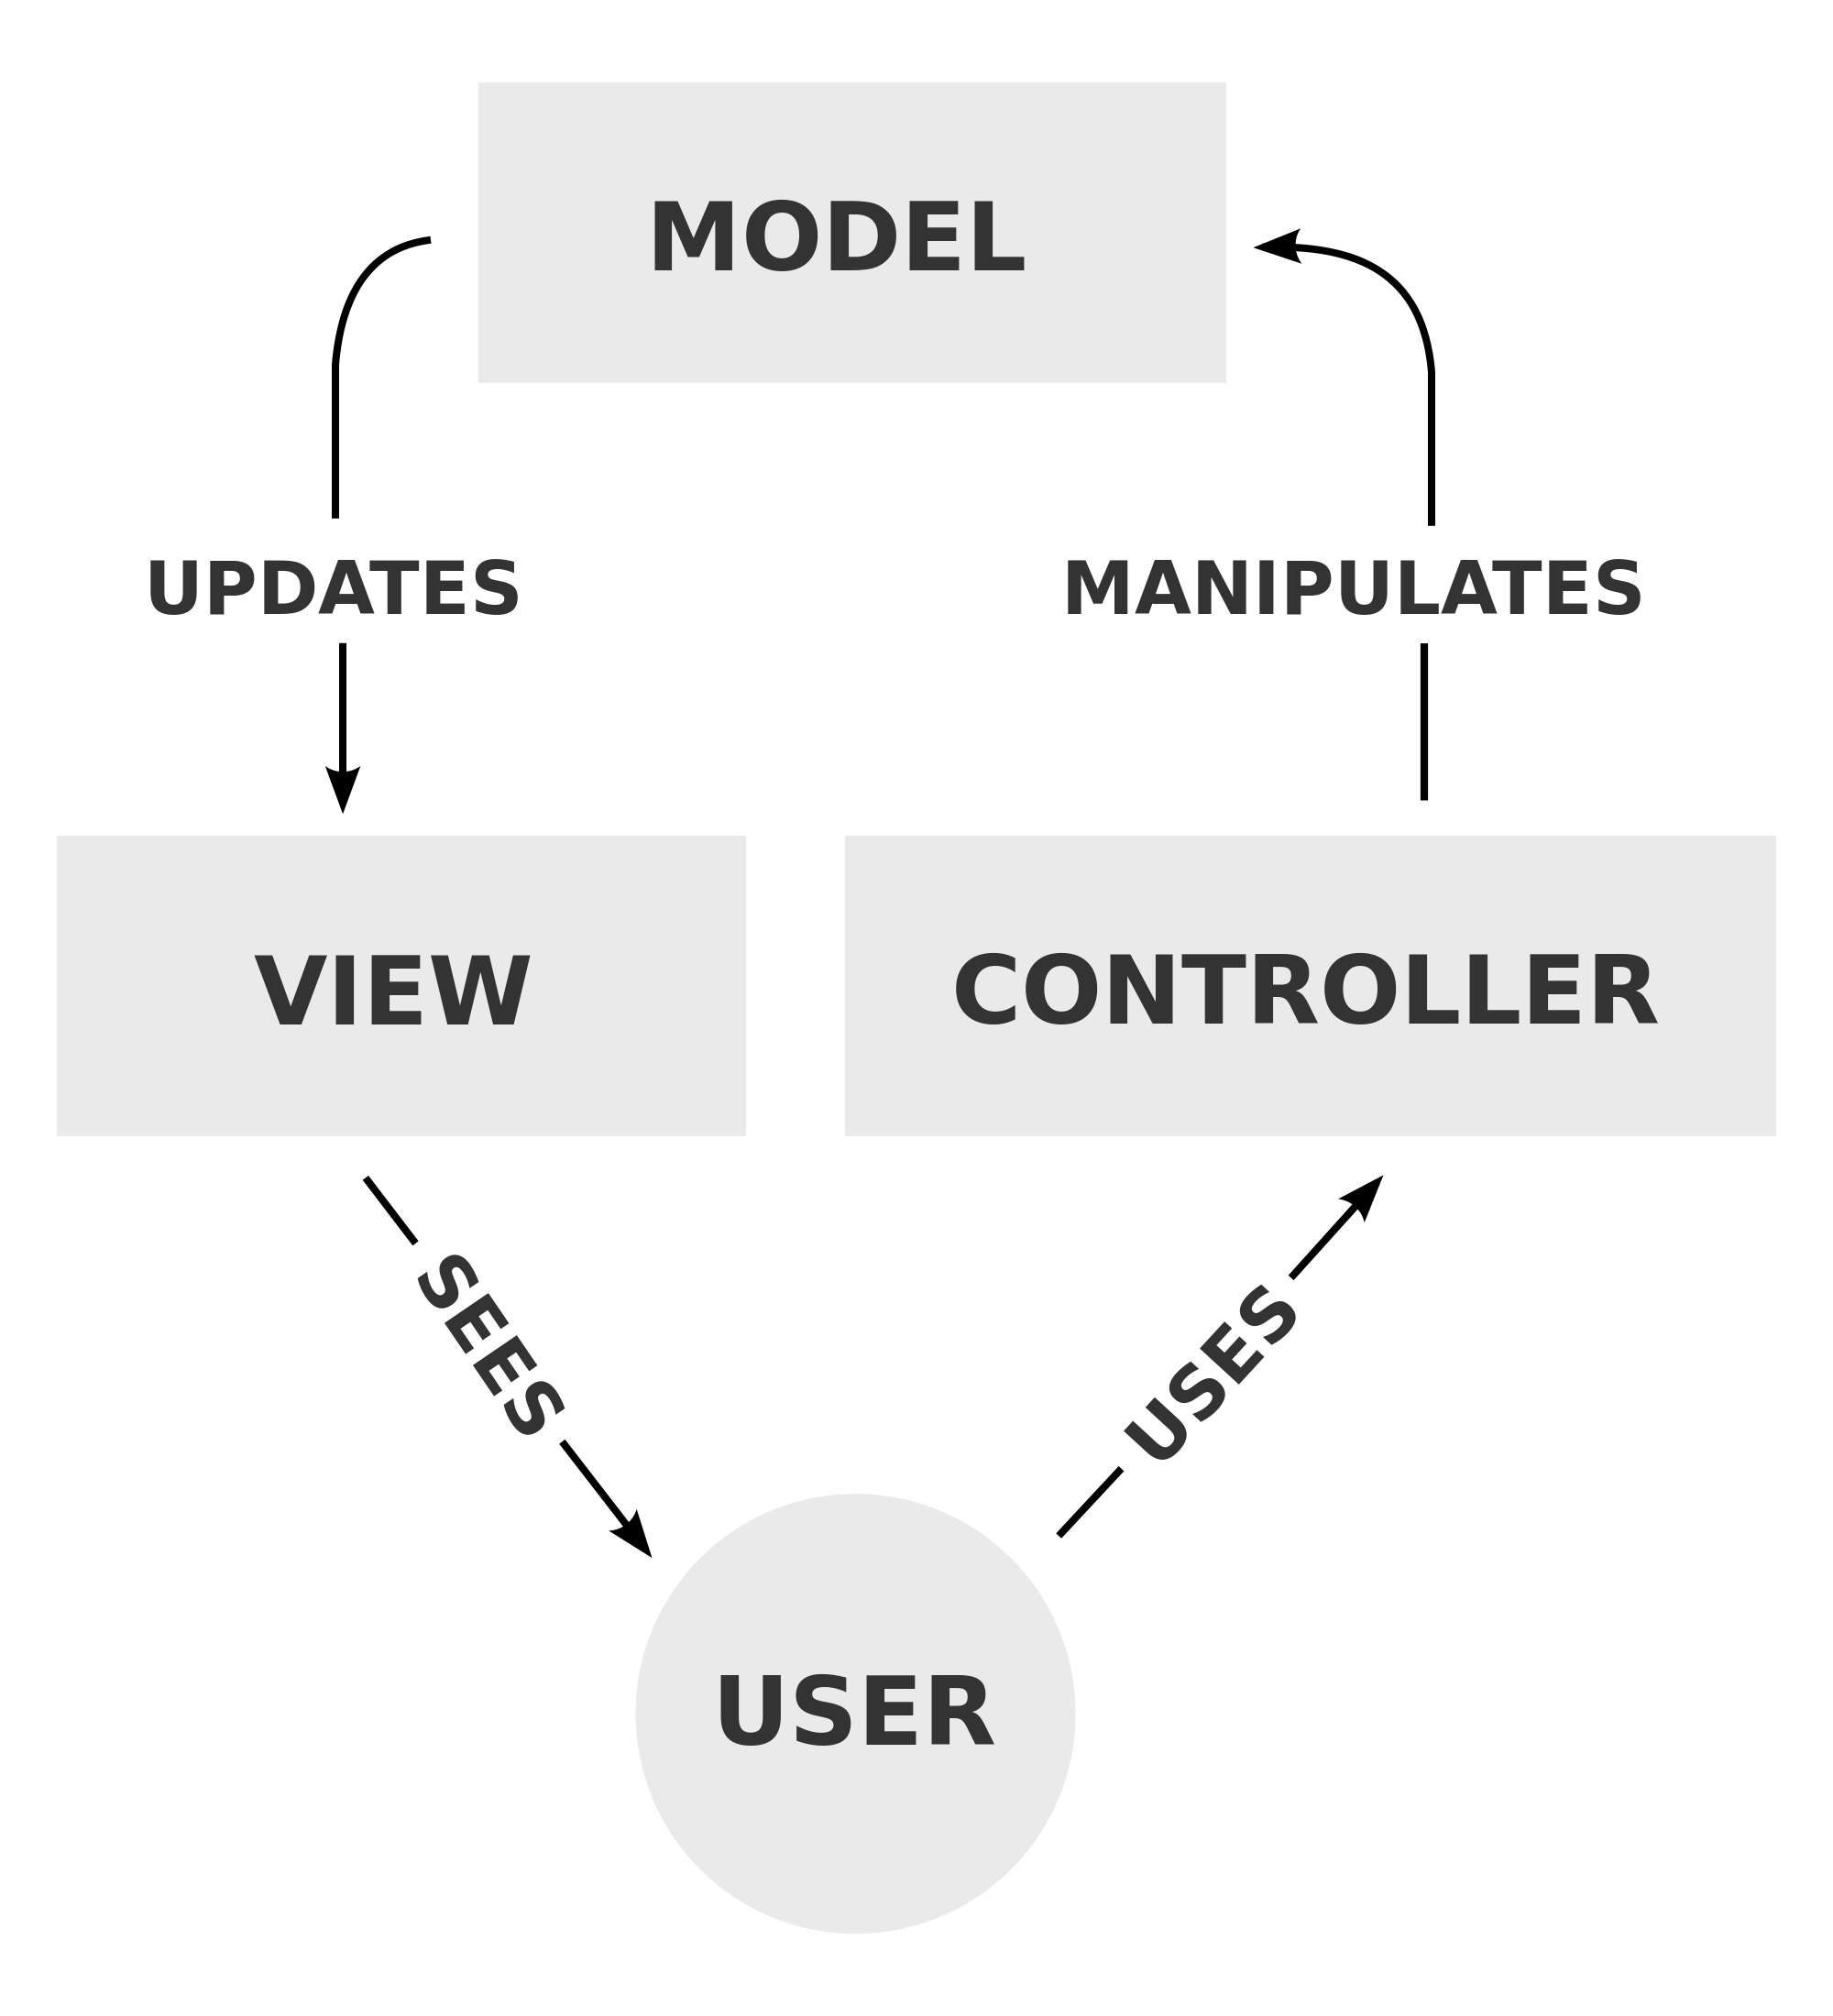
\includegraphics[width=0.5\textwidth]{img/mvc.png}
\end{figure}


\section{Spring application}

\subsection{Boot}

Talk about Spring application boot.

\subsection{Annotations...}

Parler du système d'annotations

\subsubsection{@Autowired}
Annotation présente un peu partout, on doit l'expliquer ici





\section{Application structure}

\subsection{Configuration}


\subsection{Controllers}

\subsection{Hibernate and Models}

The DAO are the link between the program and the database. There are managed by the Hibernate technology, coded in JAVA.
In fact, we have one DAO per entity (switchboard, company...), those files contains functions which returns informations from the database.
\\
\\
Hibernate simplify the interaction with the database, we don't have to use standard SQL interaction.
It works with java object and an hibernate session, we use annotation in the Java class to describe the reproduction of this object in the database,
and we can manipulate this object, transfer it by the session and it will be save on the database.



\subsection{View}

The .twig files are an evolution of the HTML files, there are managed by pebble and represents the view of the website.
A .twig file can represent a file, or a part of a file (a layout), like a that we don't have to code every time the same code (like the menu...)
.twig offer something more than a classical html file, it allow to use Java object inside the view, so we can transfer a list and process it directly inside the view.




\subsection{Services}

\subsection{Converters}
\subsection{DTO and Validator}

\subsection{Exceptions}


Due to our inability to make a real design, we chose to download a free open-source design. We found the excellent \textit{AdminLTE2} template suitable for a website like our.
\newline

We cleared and adapted it to our website and needs.
This template is based on the Bootstrap framework which ease the front-end development of a website. Furthermore, the Bootstrap framework is a responsive design: it means our website will be functional on every platform (phone, tablets, computer...) and for all screens size.

\begin{figure}[!ht]
  \caption{AdminLTE2.}
  \centering
    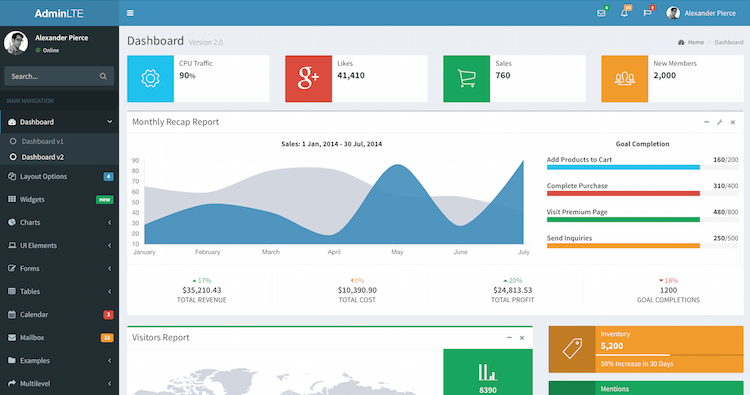
\includegraphics[width=0.9\textwidth]{img/design.png}
\end{figure}







